\chapter{Introduction}
\label{chapter:introduction}

% The page numbering must be reset here inside the file
\pagenumbering{arabic}
\setcounter{page}{1}


\section{Aim and scope of this document}
\label{sec:aim}

The sub-millimetre radiometer (\SMR\ ) onboard the Odin satellite
performs limb sounding measurements of the atmosphere.
The basic output of \smr\ is spectra in different frequency
bands, mainly within the 486\,--\,504\,GHz and 541\,--\,581\,GHz region.
After calibration, a group of such spectra can be used
to retrieve profiles of e.g. \chem{O_3}, \chem{ClO}, \chem{N_{2}O}, \chem{HNO_{3}}, 
\chem{H_{2}O}, \chem{CO}, and isotopologues of \chem{H_{2}O}, and \chem{O_{3}},
which are species that are of interest for studying stratospheric and 
mesospheric chemistry and dynamics. 

The processing of data from basic instrumental data to the
desired species concentration product involves a number of steps.
It is standard practise to divide data products into different levels, such  as:

\begin{itemize}

\item Level0 data: time tagged and sorted science and house-keeping data
as well as orbit and pointing data in separate files

\item Level1B data: groups of spectra, calibrated both in intensity and frequency. 
Pointing and instruments settings included.

\item Level2 data: extracted geophysical data (i.e. geolocated profile
of ozone concentration) from observed spectra

\end{itemize}


The aim of this document is to review and describe basic
data (Level0) from \smr\ and the algorithms used to 
to processes Level0 data into gelocated and calibrated 
groups of spectra (scans), which is refered to as Level1B data. 
The aim is also to describe the Level1B data format and 
the quality of the data.

This document is organised as follows:
\smr\ observations and measurement modes are described 
in Chapter~1. The calibration procedure is presented in
Chapter~2, and the Level1B data format, including description
of quality flags, is described in Chapter~3.
Finally,
Chapter 4 gives a summary with focus on the most important points to correctly
understand the \smr\ Level1B data. 
   

\section{Odin}

The Odin satellite was launched on 2001-02-20 into a sun-synchronous
18:00 hour ascending node orbit, carrying two co-aligned limb sounding
instruments: OSIRIS (optical spectrograph and infrared imaging system) and
\SMR\ (sub-millimetre radiometer). Originally, Odin was used for both
atmospheric and astronomical observations, however, since 2007 its only active
mission is its aeronomy. Odin is a Swedish-led project in cooperation with Canada,
France and Finland. Both of Odin's instruments are still functional, and the
present operation of the satellite is partially performed as an ESA third party
mission.
Odin passes the ground station at Esrange about 14 times each day
and raw science and house-keeping data are downloaded at
Esrange and transferred to a data archive housed by the Parallel
Data Centre (PDC) at the Royal Institute of Technology (KTH)
in Stockholm.


\subsection{The \SMR\ instrument}


%\begin{table}
%\caption{ \smr\ frontend and backend frequency specification.}
%\label{table:config}
%\begin{tabular}{|l|l|l|l|l|}
%  \hline
%  \textbf{Frontend} & \textbf{Tuning range} & \textbf{Backend} & \textbf{Bandwidth } & \textbf{Channel spacing} \\
%                    & {[}GHz{]}             &                  & {[}MHz{]}           & {[}MHz{]}\\
%  \hline
%  549 A1            & 541--558             & AOS              & 1050                & 0.61\\
%  \hline
%  495 A2            & 486--504             & AC1/AC2          & 800                 & 1.0
% \\
% \cline{1-1}
% \cline{2-2}
% \cline{4-4}
% \cline{5-5}
%  555 B2           & 547--564              &                 & 400                  & 0.5 \\
% \cline{1-1}
% \cline{2-2}
% \cline{4-4}
% \cline{5-5}
% 572 B1            & 563--581              &                 & 200                  & 0.25 \\
% \cline{1-1}
% \cline{2-2}
% \cline{4-4}
% \cline{5-5}
%  119 C           &  118.75                 &                 & 100                 & 0.125 \\
%\hline
%\end{tabular}
%\end{table}


\begin{table}
\caption{ \smr\ frontend frequency specification.}
\label{table:config1a}
\begin{tabular}{|l|l|}
  \hline
  \textbf{Frontend} & \textbf{Tuning range {[}GHz{]} } \\
  \hline
  549 A1            & 541--558              \\
  \hline
  495 A2            & 486--504              \\
  \hline
  555 B2            & 547--564             \\
 \hline
 572 B1             & 563--581              \\
 \hline
  119 C             &  118.75               \\
\hline
\end{tabular}
\end{table}



\begin{table}
\caption{ \smr\ backend frequency specification.}
\label{table:config1b}
\begin{tabular}{|l|l|l|}
  \hline
  \textbf{Backend} & \textbf{Bandwidth {[}MHz{]}} & \textbf{Channel spacing {[}MHz{]}} \\
  \hline
  AOS              & 1050                & 0.61\\
  \hline
  AC1/AC2          & 800                 & 1.0
 \\
 \cline{2-2}
 \cline{3-3}
                   & 400                  & 0.5 \\
 \cline{2-2}
 \cline{3-3}
                   & 200                  & 0.25 \\
 \cline{2-2}
 \cline{3-3}
                   & 100                 & 0.125 \\
\hline
\end{tabular}
\end{table}


%Key elements of
%SMR are a 1.1 m telescope and four tunable single-sideband
%Schottky-diode heterodyne receivers that passively measure
%the limb thermal emission in the spectral range of 486–
%581 GHz, as well as two high-resolution auto-correlator
%spectrometer
\begin{figure}[t]
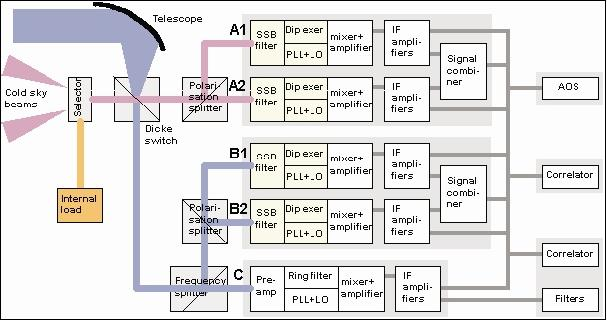
\includegraphics[width=14cm]{Odin_Auto2.jpg}
\caption{\smr\ block diagram.}
\label{fig:blockdiagram}
\end{figure}




The \smr\ package is highly tunable and flexible \citep{frisk:theod:03}.
\smr\ is equipped with one mm and four sub-mm receivers.
The four main sub-mm receiver chains can be tuned to cover
frequencies in the ranges 486\,--\,504\,GHz and 541\,--\,581\,GHz.
Table~\ref{table:config1a} lists the receivers single sideband (SSB) tuning ranges.
Martin--Pulpett interferometers are employed to provide SSB filtering 
(with a nominal sideband suppression better than 19\,dB across
the image band) and injection into the Schottky mixers.
The local oscillators are varactor-tuned Gunn diodes followed by
doubler and tripler stages. The mixers and IF amplifiers are inside a cryostat and
cooled to approximately 130 K by a 80 K Stirling cycle cooler. The receiver
noise temperatures are around 3000 K for
the sub-millimetre channels and 600 K for the millimetre channel.

The receivers form two groups, A1+A2 and B1+B2+C, in which each group shares
a common path through the beam optics (Figure~\ref{fig:blockdiagram}). 
The main observing mode is by switching against the cold sky, between the
main beam and an unfocused sky beam. In switching mode, one group will
receive its signal via the main beam while the other sees the reference signal,
and vice versa.
The two auto-correlators (ACs) of \smr\ can be coupled to any of the front-ends
and each use up to 8 x 112 MHz bands.
Eight correlator ships provides 96 lags each.
The center IF (intermediate frequency) of each sub-band is tuneable
within a 500\,MHz wide band in 1\,MHz steps. The channel spacing
ranges from 125\,KHz in 1 band mode to 1\,MHz in 8 band mode (Table ~\ref{table:config1b}).
\smr\ can be tuned to cover a wide frequency range, but the maximum total instantaneous
bandwidth is only 1.6\,GHz. In the configuration applied for
atmospheric sounding, the channels of the ACs have a spacing of 1\,MHz.
To cover all molecular transitions of interest, a 
number of ``observation modes'' have been defined. Each observation mode makes
use of two or three frequency bands. 
%On the regular observation days it is operated in the so-called basic stratospheric 
%mode with target gases \chem{O_3}, \chem{ClO}, \chem{N_{2}O}, and \chem{HNO_{3}},
%at frequncy bands around 501 and 544\,GHz.
Definition of frequency modes are found in Tables~\ref{table:config2}, 
~\ref{table:config3}, and~\ref{table:config4}, in Appendix A.
%Single sideband operation is obtained by tunable Martin-Pupplet
%interferometers. The nominal sideband suppression is better than 19\,dB across
%the image band.

\smr\ has also a receiver chain around the 118\,GHz oxygen transition which was
heavily used during Odin's astronomy mission. For the atmospheric mission, this
front-end was planned to be used for retrieving temperature profiles, but a
technical problem (drifting LO frequency) and the fact that the analysis
requires treatment of Zeeman splitting have given these data low priority. 

The main reflector of \smr\ has a diameter of 1.1\,m, giving a
vertical resolution at the tangent point of about 2\,km. 
Vertical scanning is achieved by a rotation of the satellite
platform, by an advanced attitude control system (ACS). 
The ACS uses star trackers as the main sensors with backup from gyros, 
magnetometers, and Sun sensors. Reaction wheels and magnetic coils serve as 
actuators. The ACS pointing accuracy in limb-scanning mode is 5\(^{'}\) in
real time knowledge, and better than 1\(^{'}\) in reconstructed knowledge
(which translates to a \(\sim\)800\,m vertical accuracy in tangent point).
Measurements are generally performed along the orbit plane, providing a
latitude coverage between 82.5$^{\circ}$S and 82.5$^{\circ}$N. Since the end of
2004 Odin also points off-track during certain periods, e.g.\ during the
austral summer season, allowing the latitudinal coverage to be extended towards
the poles. 




\subsection{Measurement sequence}

\begin{table}
\caption{Main scanning modes.}
\label{table:scanpattern}
\begin{tabular}{|l|l|}
  \hline
  \textbf{Scanning mode} & \textbf{Scanning range {[}km{]}} \\
  \hline
  Stratospheric scan     &  7--72 \\
 \hline
 Stratospheric/mesospheric scan &  7--110  \\
 \hline
 Summer mesospheric scan & 60--100 \\
 \hline
\end{tabular}
\end{table}


The vertical scanning of \smr`s line of sight is achieved by
rotation of the platform with a rate matching a vertical speed of
the tangent altitude of 750\,m/s. Measurements are performed during
both upward and downward scanning. The lower end of the scan is typically
at about 7\,km, and the upper end varies between 70 and 110\,km depending on
the observation mode (see Table~\ref{table:scanpattern}).

For calibration purposes, \smr\ performs aeronomy observation
in a switching mode, i.e. switching between the main beam and
an unfocused sky beam of 4.4$^{\circ}$ FWHM at all wavelengths. This is done
by means of a chopper wheel. An internal selection mirror
can choose between two possible directions of the sky beam,
separated by 28$^{\circ}$. The separation from the main beam
amounts to 42$^{\circ}$.
The selection mirror may also direct the beam towards an internal
load at ambient temperature (approximately 285 K), made of carbon 
loaded polyethylene tiles, optimised for reflecting less than -30\,dB at 500\,GHz.
%The temperature of the material is known better than 0.2 K using 
%redundant integrated temperature sensors.



\section{Further reading}
\label{sec:reading}

\citet{murtagh:anove:02} give an overview of the Odin aeronomy mission, as well
as the general technical details of \smr. \citet{frisk:theod:03} give a description
of the technical details of \smr.


